\begin{figure}
	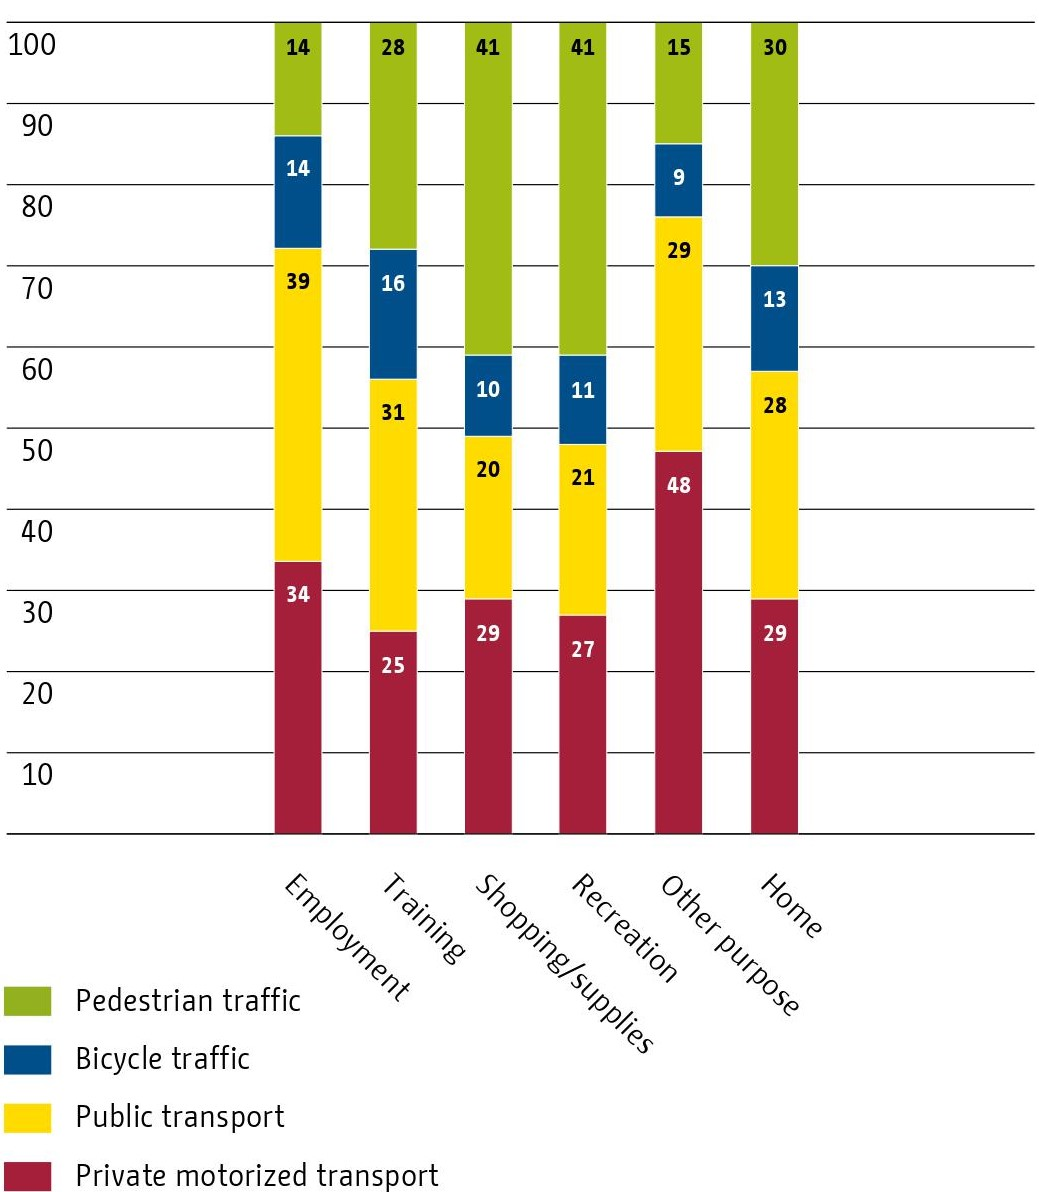
\includegraphics[width=0.5\textwidth]{MobilityInTheCityJPG/Graphs/UseOfTransportPurpose.jpg}
	\centering
	\caption{Use of transport mode by purpose of journey.\cite{MobilityCity}}
\end{figure}
\section{Car}
With a length of approximately 5400 km of roads the car remains the most used mean of transport to commute to work. Improving the roads and making more parking spaces available makes the car an atractive option. However, only 20\% of the road vehicles traveling in Berlin are private cars. The other 80\% cars are vehicles belonging to flexible, non-binding schemes and with a fixed pick-up point.  The main traffic roads\footnote{Main traffic roads: they have a total length of 160 km.} ensures that people coming from Berlin's suburbs or nearby cities reach the minor roads efficiently. The vast majority of these minor roads (370 km) have a speed limit of 30 km/h upon them, which is due to safety reasons and noise control. 

The demand for parking spaces is significantly higher than the supply, but this is where Berlin's parking policy plays a big role. A 100,000 parking spaces across 45 parking zones provides a reasonable amount of place to store the commuters vehicle during day or night. Nevertheless parking in Berlin can get expensive. If you live in Berlin and you want to park in your neighbourhood you need a permit\footnote{In German: Bewohnerparkausweis} which costs €20.40 and is valid for two years. Otherwise you have to pay at the parking meter. Outside the \textit{Ringbahn}\footnote{Berliner Ringbahn: a 37.5 km long circle route around Berlin's inner area, on the Berlin S-Bahn network.} you can park for free. Other costs like car insurance (€100 to €1000 per year), vehicle tax\footnote{Kraftfahrzeugsteuer} (around €100 per year), fuel, avehicle inspections per two years (€100), maintenance and repairs make the use of the car for commuting an expensive option.





\section{Bus}


\section{Train}


\section{Tram}


\section{Bike}


\section{Sharing systems}

